\chapter{Experiments in Simulation}
\label{maintwo}

\section{Simulation Setup} \label{sec:sim_setup}
The experiments in this thesis 
are conducted in a drone racing simulation,
which includes the environment, 
the racetrack consisting of race gates 
and the drone.
The implementation of the simulation (see figure \ref{fig:simulation_setup})
is separated into physics modeling and image rendering.
\begin{figure}%[h]
    \centering
    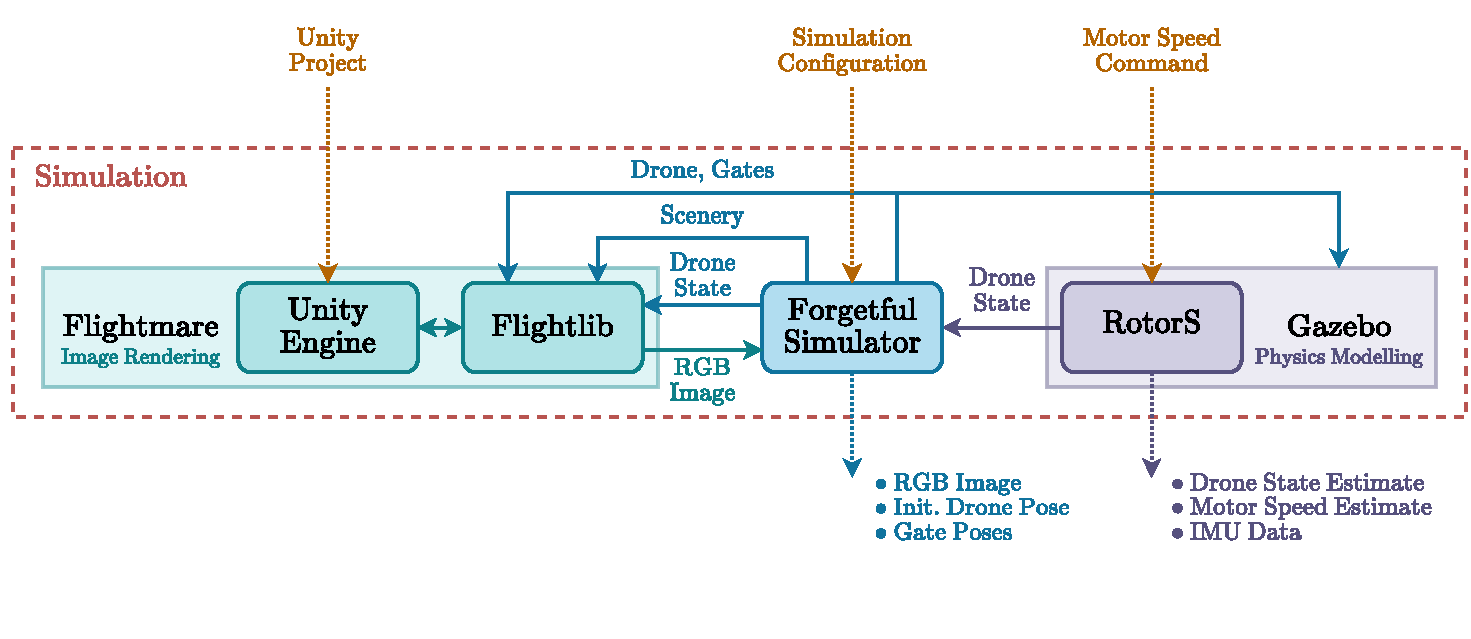
\includegraphics[width=1.0\textwidth]{own/simulation_setup.drawio.pdf}
    \caption[
        Implementation concept of the simulation
    ]{
        Implementation concept of the simulation
    \label{fig:simulation_setup}
    }
\end{figure}

For a physics modeling of high accuracy,
the Gazebo\footnote{\url{https://gazebosim.org/home}, visited on 18/08/2022} 
simulator
with the RotorS \cite{Furrer2016} plugin is deployed.
The modeling includes the dynamics of the drone under 
the actuation with inputted motor speed commands
and possible collisions of the drone with the racetrack gates.
Further, the RotorS plugin provides the
drone state estimate, the motor speeds estimate and the
data from the onboard IMU as output.


For an almost photo-realistic image rendering,
the Flightmare \cite{Song2020} simulator 
is deployed.
Upon request, the Flightlib interface
updates the drone pose 
within the Unity\footnote{
    \url{https://unity.com/}, visited on 20/08/2022
} Engine
and fetches an RGB image from the drone's onboard camera.
Before running the simulation,
the Unity Engine is built from a Unity project
that bases on the RPG Flightmare Unity Project\footnote{
    \url{https://github.com/uzh-rpg/flightmare_unity}, visited on 20/08/2022
}.
The Unity project of this thesis
entails five scenes named
spaceship interior\footnote{
    based on "3D Free Modular Kit" from the Unity Asset Store
},
destroyed city\footnote{
    based on "Destroyed City FREE" from the Unity Asset Store
},
industrial site\footnote{
    based on "RPG/FPS Game Assets for PC/Mobile (Industrial Set v2.0)" from the Unity Asset Store
},
polygon city\footnote{
    based on "CITY package" from the Unity Asset Store
}
and desert mountain\footnote{
    based on "Free Island Collection" from the Unity Asset Store
}
(see figure \ref{fig:unity_scenes}).
Within each scene, there are three sites (A, B, C) to place a racetrack.
For the racetrack, two different gate types are provided:
the first with TU Berlin/DAI-Labor logos and 
the second with Tsinghua University/DME logos
(see figure \ref{fig:unity_gates}).
\begin{figure}
    \centering
    \subfloat[
        Spaceship Interior
    ]{
        \label{fig:unity_scene_SI}
        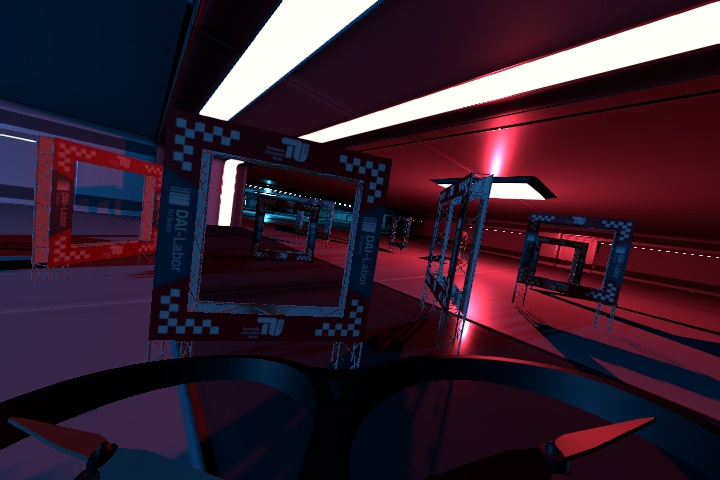
\includegraphics[width=0.33\textwidth]{own/jpg/spaceship_interior.jpg}
    }
    %\hspace*{0cm}                
    \subfloat[
        Destroyed City
    ]{
        \label{fig:unity_scene_DC}
        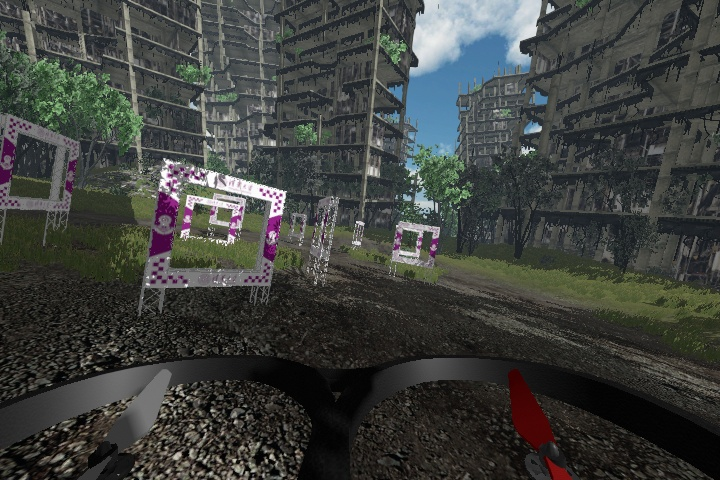
\includegraphics[width=0.33\textwidth]{own/jpg/destroyed_city.jpg}
    }
    \par
    \subfloat[
        Industrial Site
    ]{
        \label{fig:unity_scene_IS}
        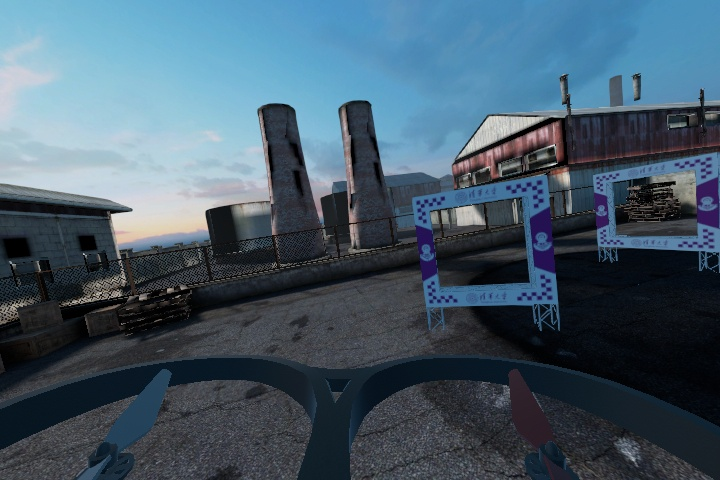
\includegraphics[width=0.33\textwidth]{own/jpg/industrial_site.jpg}
    }
    \subfloat[
        Polygon City
    ]{
        \label{fig:unity_scene_PC}
        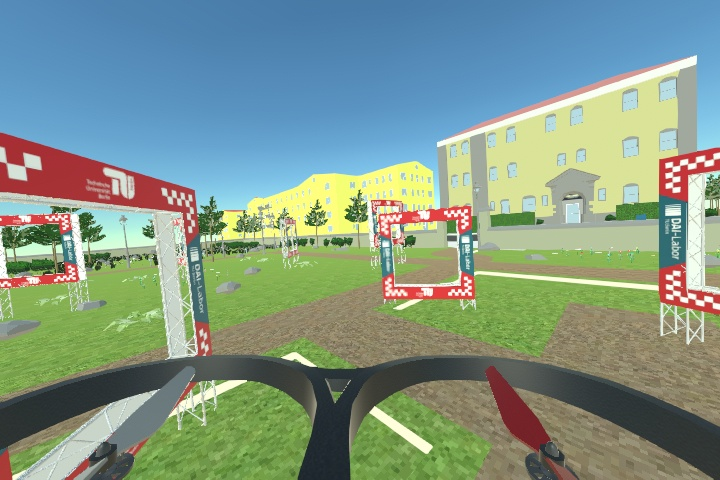
\includegraphics[width=0.33\textwidth]{own/jpg/polygon_city.jpg}
    }
    \subfloat[
        Desert Mountain
    ]{
        \label{fig:unity_scene_DM}
        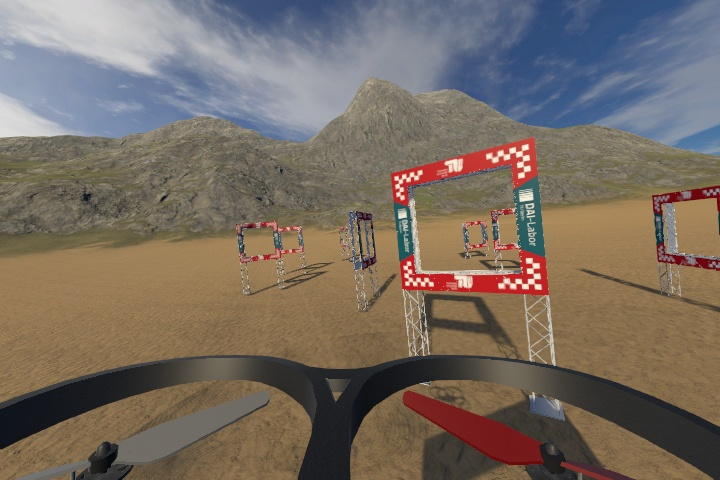
\includegraphics[width=0.33\textwidth]{own/jpg/desert_mountain.jpg}
    }
    \caption[
        Scenes available in simulation
    ]{
        Scenes available in simulation
        \label{fig:unity_scenes}
    }
\end{figure}
\begin{figure}[h]
    \centering
    \subfloat[
        DAI-Labor at TU Berlin
    ]{
        %\label{fig:unity_scene_SI}
        
\includegraphics[width=0.33\textwidth]{own/jpg/tub_dai_gate.png}
    }       
    \subfloat[
        DME at Tsinghua University
    ]{
        %\label{fig:unity_scene_DC}
        
\includegraphics[width=0.33\textwidth]{own/jpg/thu_dme_gate.png}
    }
    \caption[
        Race gates available in simulation
    ]{
        Race gates available in simulation
        \label{fig:unity_gates}
    }
\end{figure}

The Forgetful Simulator node takes on two tasks.
First, it synchronizes the
drone state in the Flightmare simulator with the
ground-truth state in the Gazebo simulator and 
provides the RGB images fetched from the Flightmare simulator
as as output.
Second, the node sets up the simulation
according to the inputted 
simulation configuration.

A simulation configuration 
includes the environment and the racetrack configuration.
The environment configuration specifies
the scene and the site.
The racetrack configuration
specifies the 
racetrack type, the racetrack generation,
the racetrack direction and the racetrack gates.
Table \ref{tab:sim_config_opts} shows all available options for the simulation configuration.
\begin{table}[h]
    \caption{Available options for the simulation configuration
    \label{tab:sim_config_opts}}
    \centering
    \begin{tabular}{|c|c|c|p{6cm}|} \hline
        \multirow{8}{*}{Simulation} 
        &\multirow{4}{*}{Environment}   
        &\multirow{3}{*}{Scenes}
        &Spaceship interior, destroyed city, industrial site, polygon city, desert mountain    
        \\\cline{3-4}
        &
        &Sites
        &A, B, C
        \\\cline{2-4}
        &\multirow{4}{*}{Racetrack}
        &Types
        &Figure-8, gap                                                                         \\\cline{3-4}
        &
        &Generations
        &Deterministic, randomized
        \\\cline{3-4}
        &
        &Directions
        &Counterclockwise, clockwise
        \\\cline{3-4}
        &
        &Gates
        &TUB-DAI, THU-DME
        \\\hline
    \end{tabular}
\end{table}
The Forgetful Simulator node stores 
the gate poses for both 
deterministic and counterclockwise
racetrack types
(see table \ref{tab:gate_pos}).
If specified,
these poses are randomized
and redirected from counterclockwise to clockwise
as illustrated in figure \ref{fig:racetrack_comp}.
The racetrack randomization 
%starts from the stored gate poses of the specified racetrack type and 
includes the following steps.
\begin{enumerate}
    \item Sample the y-position values 
    of the gates \#3-6 from the uniform real distribution
    over the intervals specified in table \ref{tab:gate_pos}.
    This step only applies to the gap racetrack type
    as it explicitely randomizes the gap distance.
    \item Shift the gate positions along the $x$-, $y$- and $z$-axis
    by a value, which is sampled
    independently for each gate and axis
    from the uniform real distribution
    over the user-specified interval 
    $\left[
        \text{-}\dist[\user]{\text{sim}}{\text{shift},\mxm}{}{},
        \dist[\user]{\text{sim}}{\text{shift},\mxm}{}{}\right]$.
    \item Scale the gate positions by a value,
    which is sampled once for all gates from the uniform real distribution
    over the user-specified interval
    $\left[
        \dist[\user]{\text{sim}}{\text{shift},\mnm}{}{}, 
        \dist[\user]{\text{sim}}{\text{shift},\mxm}{}{}\right]$.
    \item Twist the gate yaw-orientations
    by a value, which is sampled 
    independently for each gate 
    from the uniform real distribution
    over the user-specified interval
    $\left[
        -\dist[\user]{\text{sim}}{\text{twist},\mxm}{}{},
        \dist[\user]{\text{sim}}{\text{twist},\mxm}{}{}\right]$.
\end{enumerate}
After processing the racetrack configuration,
the Forgetful Simulator node computes
the start position of the drone so that
the drone is located between the second last and the last gate
and faces towards the last gate.
Then, the node loads the 
environment configuration
in the Flightmare Simulator 
and 
spawns the drone model 
and the race gate models of the specified type
at the computed poses
in both, the Flightmare and the Gazebo simulator.
Finally, the node
outputs the computed gate poses.
This information is required 
to compute the global trajectory of the expert system
(see section \ref{sec:expert_system})
and to automatically update the drone's progress on the racetrack
whenever the drone has passed the currently targeted race gate.





\begin{figure}[h]
    \newcommand{\dimmm}{0.42\textwidth}
    \newcommand{\dimmmb}{0.1\textwidth}
    \newcommand{\vertspace}{-3ex}

    \centering
        \subfloat{\footnotesize \textbf{$\downarrow$ shift}}
    \\[\vertspace]
        \subfloat{
            %\fbox{
                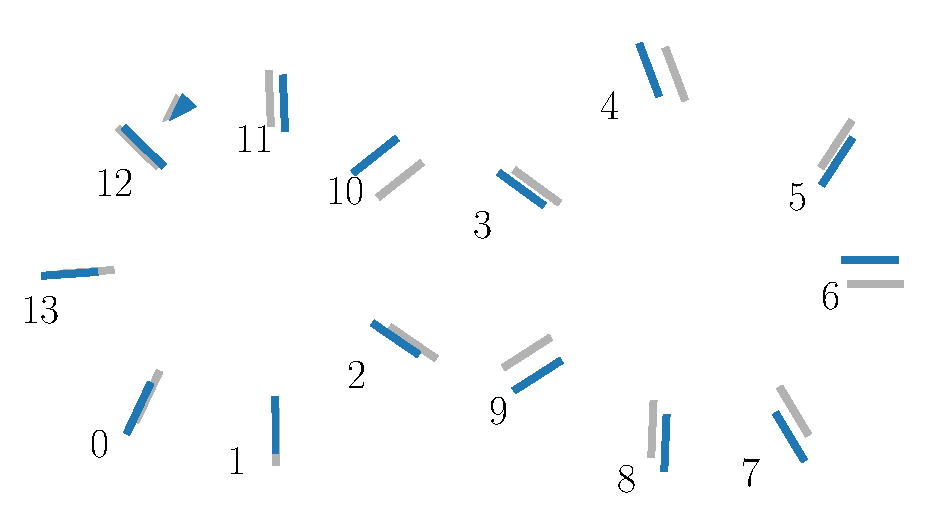
\includegraphics[width=\dimmm]{own/computeRacetrack_fig8_shift.pdf}
            %}
        }
        \subfloat{\begin{minipage}[c]{\dimmmb}$\ $\end{minipage}}
        \subfloat{
            %\fbox{
                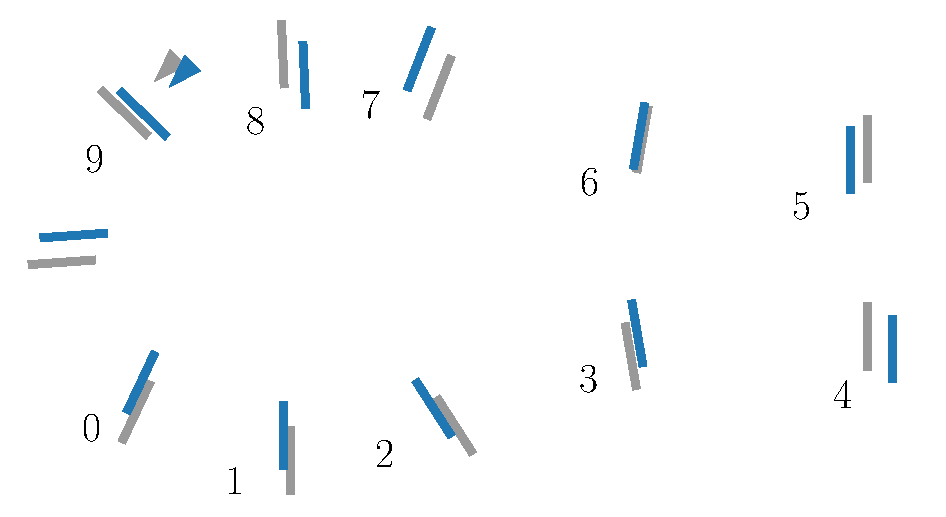
\includegraphics[width=\dimmm]{own/computeRacetrack_gap_shift.pdf}
            %}
        }
    \\[\vertspace]
        \subfloat{\footnotesize \textbf{$\downarrow$ scale}}
    \\[\vertspace]
        \subfloat{
            %\fbox{
                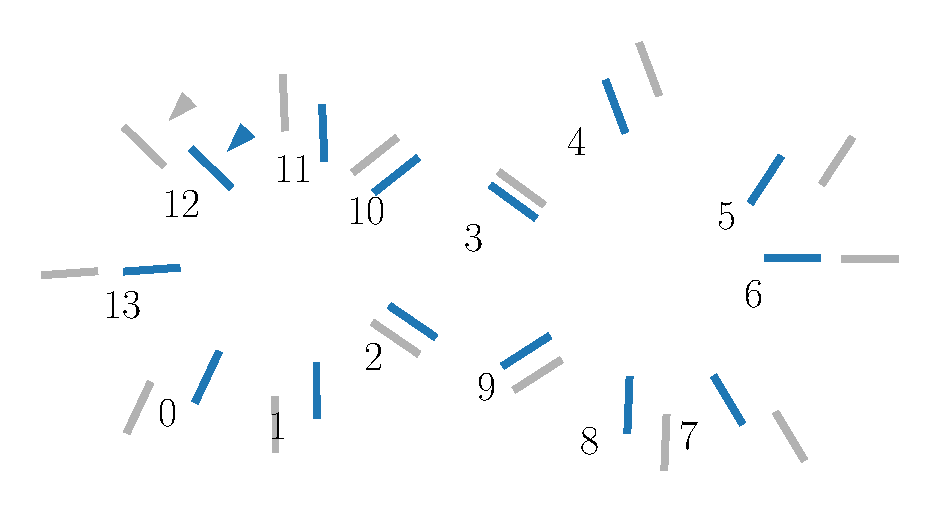
\includegraphics[width=\dimmm]{own/computeRacetrack_fig8_scale.pdf}
            %}
        }
        \subfloat{\begin{minipage}[c]{\dimmmb}$\ $\end{minipage}}
        \subfloat{
            %\fbox{
                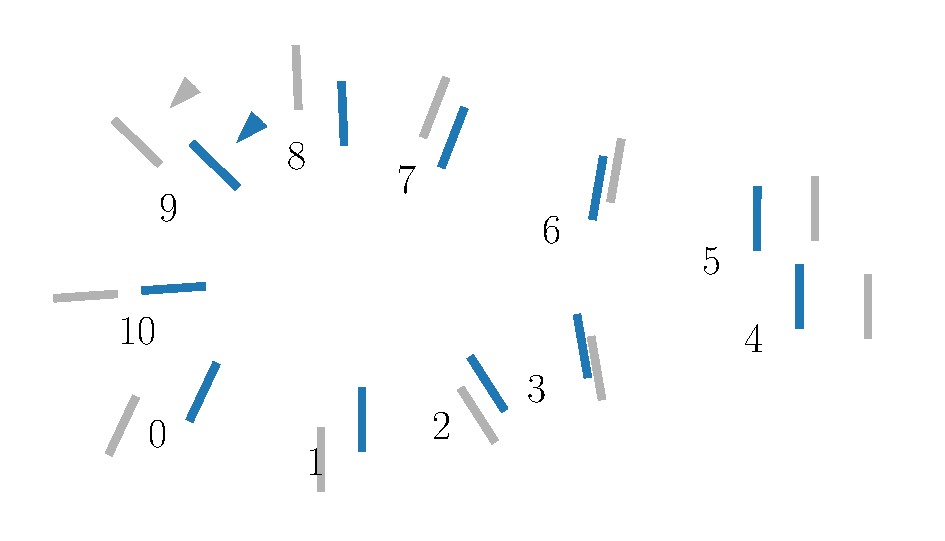
\includegraphics[width=\dimmm]{own/computeRacetrack_gap_scale.pdf}
            %}
        }
    \\[\vertspace]
        \subfloat{\footnotesize \textbf{$\downarrow$ twist}}
    \\[\vertspace]
        \subfloat{
            %\fbox{
                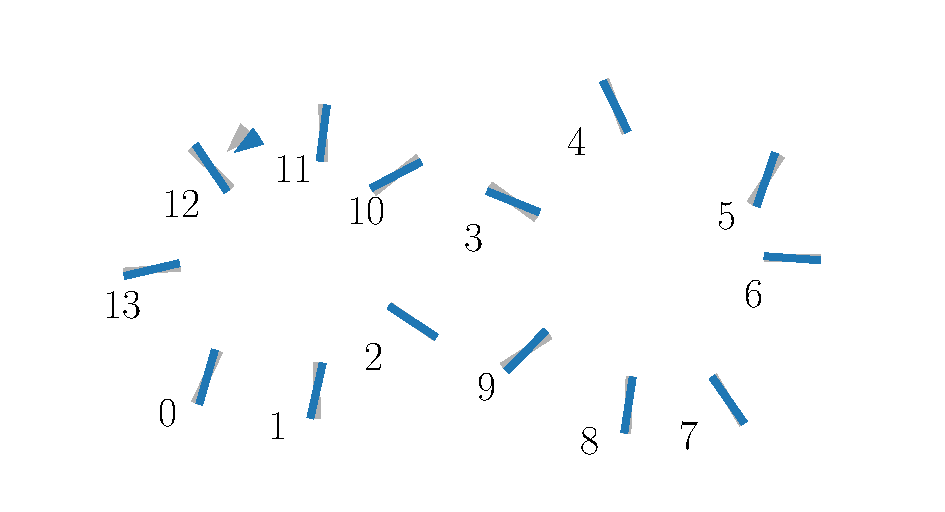
\includegraphics[width=\dimmm]{own/computeRacetrack_fig8_twist.pdf}
            %}
        }
        \subfloat{\begin{minipage}[c]{\dimmmb}$\ $\end{minipage}}
        \subfloat{
           %\fbox{
            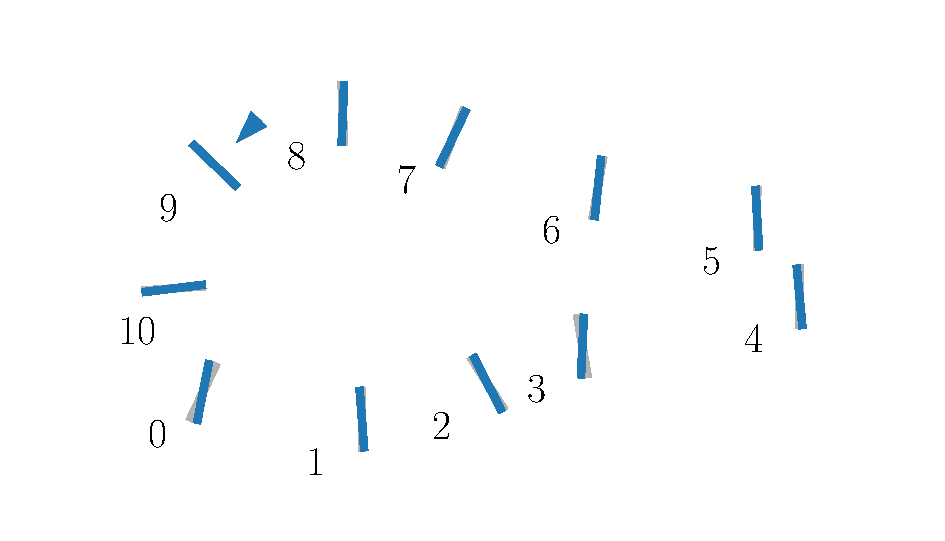
\includegraphics[width=\dimmm]{own/computeRacetrack_gap_twist.pdf}
        %}
        }
    \\[\vertspace]
        \subfloat{\footnotesize \textbf{$\downarrow$ redirect}}
    \\[\vertspace]
    \subfloat{
        %\fbox{
            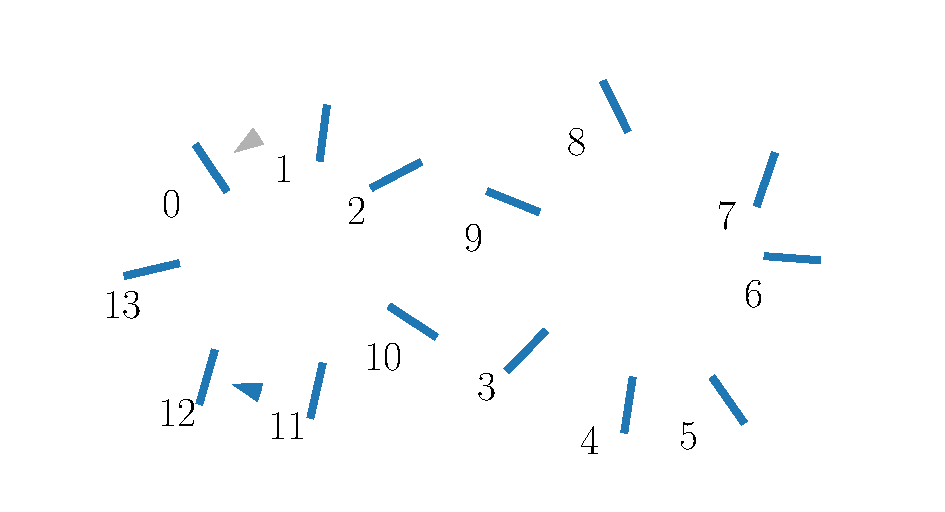
\includegraphics[width=\dimmm]{own/computeRacetrack_fig8_redir.pdf}
        %}
    }
    \subfloat{\begin{minipage}[c]{\dimmmb}$\ $\end{minipage}}
    \subfloat{
        %\fbox{
            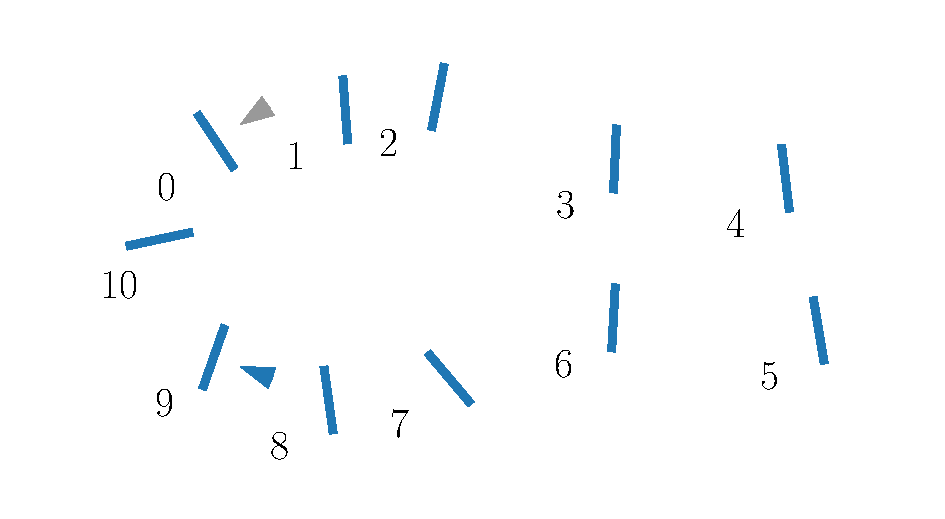
\includegraphics[width=\dimmm]{own/computeRacetrack_gap_redir.pdf}
        %}
    }
    \caption[
        Racetrack randomization and redirection
    ]{
        Racetrack randomization and redirection for
        the figure-8 (left) 
        and the gap (right) racetrack type.
        In the xy-plane, the drone starting pose (arrow) and the gate poses 
        (numbered bars)
        are shown before (grey) and after (blue) the individual processing step.
        The first randomization step, which is exclusive to the gap racetrack type,
        is not depicted.
        \label{fig:racetrack_comp}
    }
\end{figure}







\begin{table}[h]
    \footnotesize
    \caption{Deterministic gate poses\label{tab:gate_pos}}
    \centering
    \begin{tabular}{|l|l|l|l|l|l|}
    %\hline
    %\multicolumn{3}{|c|}{Team sheet} \\
    \hline
    Racetrack & Gate & x & y & z & yaw\\ 
    \hline
    \hline
    \multirow{14}{*}{Figure-8}   
    &0 &-20.45& -8.65&2.0& 1.13\\ \cline{2-6}
    &1 &-12.55&-11.15&2.0&-1.57\\ \cline{2-6}
    &2 &-4.15 & -5.35&2.0&-0.60\\ \cline{2-6}
    &3 &3.45  &  4.25&2.0&-0.63\\ \cline{2-6}
    &4 &11.95 & 11.15&2.0&-1.21\\ \cline{2-6}
    &5 &21.85 &  6.85&2.0& 0.99\\ \cline{2-6}
    &6 &24.25 & -1.75&2.0& 0.00\\ \cline{2-6}
    &7 &19.25 & -9.55&2.0&-1.03\\ \cline{2-6}
    &8 &10.55 &-10.65&2.0& 1.53\\ \cline{2-6}
    &9 &2.85  & -5.95&2.0& 0.57\\ \cline{2-6}
    &10&-4.95 &  4.65&2.0& 0.67\\ \cline{2-6}
    &11&-12.95&  9.65&2.0&-1.53\\ \cline{2-6}
    &12&-21.05&  6.65&2.0&-0.77\\ \cline{2-6}
    &13&-24.25& -1.00&2.0& 0.07\\
    \hline
    \hline
    \multirow{14}{*}{Gap}   
    &0 &-20.45&-8.65         &2.0& 1.13\\ \cline{2-6}
    &1 &-12.55&-11.15        &2.0&-1.57\\ \cline{2-6}
    &2 &-4.15 &-9.35         &2.0& -1.0\\ \cline{2-6}
    &3 &4.85  &[-4.95, -5.95]&2.0& -1.4\\ \cline{2-6}
    &4 &16.95 &[-2.25, -5.25]&2.0& 1.57\\ \cline{2-6}
    &5 &16.95 &[2.25,   5.25]&2.0& 1.57\\ \cline{2-6}
    &6 &5.45  &[4.45,   5.45]&2.0&  1.4\\ \cline{2-6}
    &7 &-4.95 &7.95          &2.0&  1.2\\ \cline{2-6}
    &8 &-12.95&9.65          &2.0&-1.53\\ \cline{2-6}
    &9 &-21.05&6.65          &2.0&-0.77\\ \cline{2-6}
    &10&-24.25&-1.0          &2.0& 0.07\\
    \hline
    \end{tabular}
\end{table}






%\section{ANN Module Variants}
%In the experiments, several
%variants of the ANN module (see section \ref{sec:ann_module})
%are examined for their racing performance.
%Table \ref{tab:ann_module_variants} shows these variants
%and their configurations.
%The configuration of a variant
%is structured into
%input, output and the 
%CNN, GRU, FC, and HEAD submodule.
%
%The input configuration includes:
%the sequence length $\seqLen$ of the training samples 
%(see equ. \ref{eq:seq_len}),
%the resize factor $\resizeFact$ 
%of the image preprocessing (see equ. \ref{eq:rgb_preproc})
%as well as the switchable optional inputs
%$\rawRGBTimeStep$, 
%$(\IMULinAcc,\IMUAngVel)$
%and
%$\IMUTimeStep$ (see equ. \ref{eq:opt_inp_vec}).
%The output configuration includes:
%navigation decision
%$\headNavDec$ (see equ. \ref{eq:head_nav_dec})
%and control command
%$\headCtrlCmd$ (see equ. \ref{eq:head_ctrl_cmd}).
%For the
%configurations regarding the CNN, GRU, FC and HEAD submodules,
%see the corresponding paragraphs in section \ref{sec:ann_module}. 
%
%
%%All of the examined variants have three configurational aspects in common.
%%First, all available optional inputs are activated.
%%Second, navigation decisions are selected as output option.
%%Third, the CNN submodule implements the backbone of the ResNet18 PyTorch implementation
%%whose parameters are trainable and pretrained on ImageNet !!!.
%%The ResNet18 contains 18 layers and has ... trainable parameters ...
%
%\providecommand{\ncols}{}
%\renewcommand{\ncols}{5}
%\begin{table}[h]
%    \caption{ANN module variants\label{tab:ann_module_variants}}
%    \centering
%    \begin{tabular}{|l|l|l|l|l|} \hline
%                        &                           &Baseline               &Baseline+              & Sequential \\\hline\hline
%\multirow{2}{*}{Train.} &Scene                      &$\setOfInts{1,2,3,4}$  &$\setOfInts{1,2,3,4}$  &$\setOfInts{1,2,3,4}$  \\\cline{2-\ncols}
%                        &Racetrack type             &Gap                    &Gap                    &Gap                    \\\hline
%\multirow{5}{*}{Input}  &$\seqLen$                  &1                      &1                      &$\setOfInts{2,3,5,10,25}$             \\\cline{2-\ncols}
%                        &$\resizeFact$              &\sfrac{1}{2}           &\sfrac{1}{2}           &$\setOfInts{\sfrac{1}{2}, \sfrac{1}{3}}$   \\\cline{2-\ncols}
%                        &$\rawRGBTimeStep$          &\xmark                 &\cmark                 &\cmark         \\\cline{2-\ncols}
%                        &$(\IMULinAcc,\IMUAngVel)$  &\xmark                 &\cmark                 &\cmark         \\\cline{2-\ncols}
%                        &$\IMUTimeStep$             &\xmark                 &\cmark                 &\cmark         \\\hline
%\multirow{1}{*}{Output} &$\headNavDec$              &\cmark                 &\cmark                 &\cmark         \\\cline{2-\ncols}
%                        &$\headCtrlCmd$             &\xmark                 &\xmark                 &\xmark         \\\hline
%\multirow{3}{*}{CNN}    &Model                      &resnet8                &resnet18               &resnet18       \\\cline{2-\ncols}
%                        &Pretrained                 &\xmark                 &\cmark                 &\cmark         \\\cline{2-\ncols}
%                        &Trainable                  &\cmark                 &\xmark                 &\cmark         \\\hline
%\multirow{3}{*}{GRU}    &$\GRUNumLayer$             &\xmark                 &\xmark                 &3              \\\cline{2-\ncols}
%                        &$\GRUHiddenSize$           &\xmark                 &\xmark                 &16             \\\cline{2-\ncols}
%                        &$\GRUDropoutP$             &\xmark                 &\xmark                 &0.5            \\\hline
%\multirow{4}{*}{FC}     &$\fcLayer$                 &1                      &3                      &\xmark         \\\cline{2-\ncols}
%                        &$\fcOut$                   &256                    &32                     &\xmark         \\\cline{2-\ncols}
%                        &$\fcDropoutProb$           &0.5                    &0.2063                 &\xmark         \\\cline{2-\ncols}
%                        &$\fcAct$                   &ReLU                   &ReLU                   &ReLU           \\\hline
%\multirow{1}{*}{HEAD}   &$\headAct$                 &ReLU                   &ReLU                   &ReLU           \\\hline
%    
%    \end{tabular}
%\end{table}
%
%%https://en.wikipedia.org/wiki/Multiply%E2%80%93accumulate_operation
%%https://ai.stackexchange.com/questions/23482/are-mult-adds-and-flops-equivalent
%%https://github.com/TylerYep/torchinfo
%
%Table \ref{tab:ann_module_variants_nparams}
%shows the number of trainable and non-trainable parameters 
%as well as multiply-accumulate operations.
%
%
%For each variant, the num
%\begin{table}[h]
%    \caption{ANN module variants: 
%        number of trainable and non-trainable parameters 
%        and number of multiply-accumulate operations\label{tab:ann_module_variants_nparams}}
%    \centering
%    \begin{tabular}{|l|l|r|r|r|} \hline
%                        &\#                     &Baseline       &Baseline+      &Sequential \\\hline\hline
%\multirow{3}{*}{CNN}    &Trainables             &               &0              &0          \\\cline{2-\ncols}
%                        &Non-trainables         &               &11,176,512     &11,689,512 \\\cline{2-\ncols}
%                        &MAC Operations         &               &1,408,910,720  &           \\\hline
%\multirow{3}{*}{CAT}    &Trainables             &0              &0              &0          \\\cline{2-\ncols}
%                        &Non-trainables         &0              &0              &0          \\\cline{2-\ncols}
%                        &MAC Operations         &0              &0              &0          \\\hline                        
%\multirow{3}{*}{GRU}    &Trainables             &0              &0              &           \\\cline{2-\ncols}
%                        &Non-trainables         &0              &0              &           \\\cline{2-\ncols}
%                        &MAC Operations         &0              &0              &           \\\hline
%\multirow{3}{*}{FC}     &Trainables             &               &41,664         &0          \\\cline{2-\ncols}
%                        &Non-trainables         &               &0              &0          \\\cline{2-\ncols}
%                        &MAC Operations         &               &41,664         &0          \\\hline                        
%\multirow{3}{*}{HEAD}   &Trainables             &               &195            &           \\\cline{2-\ncols}
%                        &Non-trainables         &               &0              &           \\\cline{2-\ncols}
%                        &MAC Operations         &               &195            &           \\\hline\hline
%\multirow{3}{*}{Total}  &Trainables             &               &41,859         &           \\\cline{2-\ncols}
%                        &Non-trainables         &               &11,176,512     &           \\\cline{2-\ncols}
%                        &MAC Operations         &               &1,408,952,579  &           \\\hline
%
%%        CNN &n/a&\multicolumn{2}{|c|}{11,689,512}\\\hline
%%        GRU &\ref{eq:gru_param}&0&28,704\\\hline
%%        FC  &\ref{eq:fc_param}&262,144&0\\\hline
%%        HEAD&\ref{eq:head_param}&1,536&51\\\hline\hline
%%        Total&n/a&11,953,192&11,718,267\\\hline
%    \end{tabular}
%\end{table}

\section{Imitation learning process of the ANN Module} \label{sec:training}
The ANN module of the autonomous navigation method 
must first learn to make meaningful navigation decisions.
In this thesis as well as in the baseline work,
this task is viewed as an imitation learning problem.
The goal is that the ANN module learns to mimic
the navigation decision making demonstrated by the expert system
of section \ref{sec:expert_system}.
The problem is addressed with dataset aggregation,
which is a type of interactive direct policy learning
(see section \ref{sec:imitation_learning}).
In the learning process, 
rollouts to generate additional training data 
alternate with supervised trainings of the ANN module on the aggregated dataset.
During a rollout, the drone navigates through a racetrack
based on the navigation decisions of the ANN module.
Whenever the ANN module makes a navigation decision 
that would cause the drone to deviate too far from the
expert's global trajectory through the racetrack, 
the interactive expert system intervenes 
and provides an expert navigation decision that is executed instead.
Also, 
a training sample labeled with the expert navigation decision 
is added to the training dataset 
so that, during training, the ANN module can learn from the mistakes made
during rollout.


The user specifies the learning configuration
for the individual ANN module variant, 
which includes the rollout and the training configuration.
The rollout configuration comprises 
a set $\mathcal{S}$ of simulation configurations 
(see table \ref{tab:sim_config_opts}),
a set $\mathcal{V}$ of maximum drone speeds 
(see equ. \ref{eq:planning_des_speed})
and a set $\mathcal{E}$ of pairs of 
margins and thresholds for the expert intervention share
(hereafter referred to as margin-threshold pairs).
A margin determines the
distance of the drone from the global trajectory
above which the expert intervenes.
The threshold determines 
the share of expert navigation decisions 
in the total navigation decisions of a rollout, 
below which a rollout configuration is considered sufficiently learned.
The training configuration comprises 
the sequence length of the training samples aggregated during rollout
(which must be one if the individual ANN module is not recurrent),
the number of epochs after each rollout,
the batch size,
the loss function,
the optimizer type and the scheduling of the learning rate.
\begin{table}[h]
    \caption{Learning configuration
    \label{tab:learn_config}}
    \centering
    \begin{tabular}{|c|c|c|} 
        \hline
        \multirow{9}{*}{Learning} 
        &\multirow{3}{*}{Rollout}   
        &Simulation configurations $\mathcal{S}$
        \\\cline{3-3}
        &
        &Max. drone speeds $\mathcal{V}$
        \\\cline{3-3}
        &
        &Margin-threshold pairs $\mathcal{E}$
        \\\cline{2-3}
        &\multirow{6}{*}{Training}   
        &Sequence length $\seqLen$
        \\\cline{3-3}
        &
        &Number of Epochs $\num[\user]{\text{epoch}}{}{}{}$
        \\\cline{3-3}
        &
        &Batch size $\batchSize$
        \\\cline{3-3}
        &
        &Loss
        \\\cline{3-3}
        &
        &Optimizer
        \\\cline{3-3}
        &
        &Learning rate
        \\\hline
    \end{tabular}
\end{table}


In detail, the learning process proceeds in the following steps.
\begin{itemize}
    \item For every margin-threshold pair $(M,T)$ in $\mathcal{E}$
    \item For every simulation configuration $S$ in $\mathcal{S}$
    \item For every maximum drone speed $V$ in $\mathcal{V}$
\end{itemize}
\begin{enumerate}
    \item Process and load $S$ in the simulation.
    \item Set the maximum drone speed $\speed[\user]{\drone}{\mxm}{}{} = v$
    of the planning module.
    \item Compute the expert's global trajectory through the racetrack.
    \item Roll out the ANN module with the interactive expert system
    for one round on the racetrack.
    At the user-specified main frequency $\freq[\user]{\main}{}{}{}$, 
    the following steps are taken.
    \begin{enumerate}
        \item The latest data from the onboard sensors is preprocessed
        to a single (non-sequential) input.
        (Which sensor data is included depends on the configuration of the individual ANN module.)
        \item The ANN module processes the single input
        to make a navigation decision. 
        (If the individual ANN module is recurrent, it can still make temporal connections
        because the single inputs incoming at the frequency $\freq[\user]{\main}{}{}{}$
        constitute a time series.)
        \item The planning module computes the local trajectory for the ANN navigation decision.
        \item If the end position of the local trajectory 
        is more distant from the expert's global trajectory than $M$:
        %the expert system intervenes by demonstrating a navigation decision,
        %whereupon the planner recomputes the local trajectory.
        \begin{enumerate}
            \item The expert system intervenes by making a navigation decision
            based on its knowledge.
            \item The planning module re-computes the local trajectory for the expert navigation decision.
        \end{enumerate}
        \item The local trajectory is forwarded to the control stack,
        which tracks it at a higher frequency than $\freq[\user]{\main}{}{}{}$.
    \end{enumerate}
    \item For every expert intervention of the latest rollout, 
    add a sample to the training dataset.
    A sample comprises an expert navigation decision as a label
    and the corresponding sequence of inputs
    for the individual ANN module variant.
    The sequence starts $\seqLen$ timesteps 
    of duration $1/\freq[\user]{\main}{}{}{}$ 
    back in time and
    ends at the time step where
    the expert made the navigation decision.
    Record the share of the expert navigation decisions 
    in the total (expert and ANN) navigation decisions made during the rollout.
    \item Train the ANN module on the 
    aggregated training dataset with supervised learning.
    The number of epochs $\num[\user]{\text{epoch}}{}{}{}$,
    the batch size $\batchSize$,
    the loss function, the optimizer and the learning rate scheduling
    are specified in the training configuration.
    (For a recurrent ANN module, the samples of the training dataset
    are usually sequential. The ANN module then operates in many-to-one mode,
    whereby only the navigation decision from the processing of the last input 
    of the input sequence is used to calculate the loss.)
    \item If the recorded expert intervention share (from step 5) is greater
    than $T$, go back to step 1. Else the current 
    $(M,T)$-$S$-$V$ combination in the rollout configuration
    is considered as sufficiently learned by the ANN module.
\end{enumerate}

\section{Racing Tests}
After an ANN module variant completed the imitation learning process,
its racing performance is tested.
To do this, the ANN module variant is rolled out
with the expert system deactivated.
From records made during the rollout,
the variant's racing performance is evaluated.


The user specifies the testing configuration
(see table \ref{tab:test_config}),
which includes a set of simulation configurations,
a set of maximum drone speeds,
and the number $\num[\user]{\text{rep}}{}{}{}$ of rollout repetitions for a given
combination of simulation configuration and maximum drone speed.
In order to ensure comparability of the racing performance
of different ANN module variants while also using randomized racetracks,
$\num[\user]{\text{rep}}{}{}{}$ randomized racetracks are pre-computed 
for every possible simulation configuration 
(see table \ref{tab:sim_config_opts}).
\begin{table}[h]
    \caption{Testing configuration
    \label{tab:test_config}}
    \centering
    \begin{tabular}{|c|c|} 
        \hline
        \multirow{3}{*}{Testing}   
        &Simulation configurations $\mathcal{S}$
        \\\cline{2-2}
        &Max. drone speeds $\mathcal{V}$
        \\\cline{2-2}
        &number of repetitions $\num[\user]{\text{rep}}{}{}{}$
        \\\hline
    \end{tabular}
\end{table}

In detail, the racing tests are conducted as follows.
\begin{itemize}
    \item For every simulation configuration $S$ in $\mathcal{S}$
    \item For every maximum drone speed $V$ in $\mathcal{V}$
    \item For every repetition $N$ in $\mathcal{N}$
\end{itemize}
\begin{enumerate}
    \item Load $S$ with the $N$-th pre-computed racetrack for $S$ in the simulation.
    \item Set the maximum drone speed $\speed[\user]{\drone}{\mxm}{}{} = v$
    of the planning module.
    \item Roll out the ANN module for one round on the racetrack.
    At the user-specified main frequency $\freq[\user]{\main}{}{}{}$, 
    the following steps are taken.
    \begin{enumerate}
        \item Record the time-stamped position of the drone.
        \item The latest data from the onboard sensors is preprocessed
        to a single (non-sequential) input.
        (Which sensor data is included depends on the configuration of the individual ANN module.)
        \item The ANN module processes the single input
        to make a navigation decision. 
        (If the individual ANN module is recurrent, it can still make temporal connections
        because the single inputs incoming at the frequency $\freq[\user]{\main}{}{}{}$
        constitute a time series.)
        \item The planning module computes the local trajectory for the ANN navigation decision.
        \item The local trajectory is forwarded to the control stack,
        which tracks it at a higher frequency than $\freq[\user]{\main}{}{}{}$.
    \end{enumerate}
    \item Record if the drone, during the latest rollout, 
    completed the racetrack
    by traversing all gates without crashing. 
\end{enumerate}
The recordings allow the race performance 
of an ANN module variant to be evaluated.
On the basis of the racetrack completion records,
a variant's racetrack completion share,
on a set of simulation configurations 
depending on the maximum drone speed
can be calculated.
The racetrack completion share quantifies
the robustness of a variant's navigation decision making 
for a given setup.
The time-stamped drone position records of the rollouts
reproduce the flight trajectories induced by a variant.
The optimality with respect to jerk and snap
of these trajectories and therewith the 
variant's navigation decision making 
can be quantified
with the loss functions of the optimization problem formulations
of the global and the local trajectory
(see equ. \ref{eq:glo_traj_opt_prob} and \ref{eq:loc_traj_opt_prob}).









\section{Experiment 1}
Experiment 1 studies the racing performance of 
several feedforward and recurrent ANN module variants 
on the randomized, counterclockwise figure-8 racetrack
for varying maximum drone speeds.
Table \ref{tab:e1_ann_config} shows 
the configurations of the variants examined in this experiment.
\providecommand{\ncols}{}\renewcommand{\ncols}{8}
\providecommand{\wcols}{}\renewcommand{\wcols}{1.3cm}
\begin{table}[h]
    \caption{ANN Module Variants of Experiment 1\label{tab:e1_ann_config}}
    \centering
    \begin{tabular}{|c|c|c|p{\wcols}|p{\wcols}|p{\wcols}|p{\wcols}|p{\wcols}|} 
        \cline{4-\ncols}
        \multicolumn{3}{c|}{}
        &\multicolumn{2}{c|}{Feedforward}
        &\multicolumn{3}{c|}{Recurrent}
        \\\cline{4-\ncols}
        \multicolumn{3}{c|}{}
        &F1
        &F2
        &R1
        &R2
        &R3
        \\\hline
        %
        \multirow{14}{*}{\rotcell{ANN}}
        &\multirow{4}{*}{CNN}
        &Input
        &\multicolumn{5}{c|}{240x160 RGB}
        \\\cline{3-\ncols}
        %
        &&Model
        &Resnet8
        &\multicolumn{4}{c|}{Resnet14}
        \\\cline{3-\ncols}
        %
        &&Pretrained
        &\multicolumn{4}{c|}{No}
        &Yes
        \\\cline{3-\ncols}
        %
        &&Trainable
        &\multicolumn{4}{c|}{Yes}
        &Partly
        \\\cline{2-\ncols}
        %
        &\multirow{1}{*}{CAT}
        &Opt. Input
        &\multicolumn{3}{c|}{None}
        &All
        &None
        \\\cline{2-\ncols}
        %
        &\multirow{3}{*}{GRU}
        &\# Layers
        &\multicolumn{2}{c|}{\multirow{3}{*}{None}}
        &\multicolumn{3}{c|}{3}
        \\\cline{3-3}\cline{6-\ncols}
        %
        &&Hidden size
        &\multicolumn{2}{c|}{}
        &\multicolumn{3}{c|}{64}
        \\\cline{3-3}\cline{6-\ncols}
        %
        &&Dropout
        &\multicolumn{2}{c|}{}
        &\multicolumn{3}{c|}{0.00346}
        \\\cline{2-\ncols}
        %
        &\multirow{4}{*}{FC}
        &\# Layers
        &\multicolumn{2}{c|}{3}
        &\multicolumn{3}{c|}{\multirow{4}{*}{None}}
        \\\cline{3-5}
        %
        &&Width
        &\multicolumn{2}{c|}{256}
        &\multicolumn{3}{c|}{}
        \\\cline{3-5}
        %
        &&dropout
        &\multicolumn{2}{c|}{0.206299}
        &\multicolumn{3}{c|}{}
        \\\cline{3-5}
        %
        &&Activation
        &\multicolumn{2}{c|}{ReLU}
        &\multicolumn{3}{c|}{}
        \\\cline{2-\ncols}
        %
        &\multirow{2}{*}{HEAD}
        &Activation
        &\multicolumn{5}{c|}{ReLU}
        \\\cline{3-\ncols}
        &&Output
        &\multicolumn{5}{c|}{Navigation decision}
        \\\hline
    \end{tabular}
\end{table}
Table \ref{tab:e1_learn_config} shows the learning configuration 
for the variants examined in this experiment.
\providecommand{\ncols}{}\renewcommand{\ncols}{7}
\providecommand{\wcols}{}\renewcommand{\wcols}{1.0cm}
\begin{table}[h]
    \caption{Learning configuration of Experiment 1
    \label{tab:e1_learn_config}}
    \centering
    \begin{tabular}{|c|c|c|c|p{\wcols}|p{\wcols}|p{\wcols}|p{\wcols}|p{\wcols}|} 
        \cline{5-9}
        \multicolumn{4}{c|}{}
        &\multicolumn{2}{c|}{Feedforward}
        &\multicolumn{3}{c|}{Recurrent}
        \\\cline{5-9}
        \multicolumn{4}{c|}{}
        &F1
        &F2
        &R1
        &R2
        &R3
        \\\cline{5-9}\hline
        \multirow{14}{*}{\rotcell{Learning}} 
        &
        \multirow{8}{*}{\rotcell{Rollout}}
        &\multirow{2}{*}{\shortstack{Environ-\\ments}}
        &Scenes
        &\multicolumn{5}{c|}{Spaceship interior}
        \\\cline{4-9}
        &&&Sites
        &\multicolumn{5}{c|}{A}
        \\\cline{3-9}
        &&\multirow{4}{*}{\shortstack{Race-\\tracks}}
        &Types
        &\multicolumn{5}{c|}{Figure-8}
        \\\cline{4-9}
        &&&Generations
        &\multicolumn{5}{c|}{Randomized}
        \\\cline{4-9}
        &&&Directions
        &\multicolumn{5}{c|}{Counterclockwise}
        \\\cline{4-9}
        &&&Gates
        &\multicolumn{5}{c|}{TUB-DAI, THU-DME}
        \\\cline{3-9}
        &
        &\multicolumn{2}{c|}{Max. drone speeds}
        &\multicolumn{5}{c|}{4, 5, 6, 7, 8, 9, 10 m/s}
        \\\cline{3-9}
        &
        &\multicolumn{2}{c|}{Margin-threshold pairs}
        &\multicolumn{5}{c|}{(0.5, 10), (0.75, 5), (1.0 m, 1 \%)}
        \\\cline{2-9}        
        &
        \multirow{6}{*}{\rotcell{Training}}
        %\multirow{6}{*}{Training}   
        &\multicolumn{2}{c|}{Sequence length}
        &\multicolumn{2}{c|}{1}
        &\multicolumn{3}{c|}{25}
        \\\cline{3-9}
        &
        &\multicolumn{2}{c|}{\# Epochs}
        &\multicolumn{2}{c|}{10}
        &\multicolumn{3}{c|}{3}
        \\\cline{3-9}
        &
        &\multicolumn{2}{c|}{Batch size}
        &256
        &32
        &\multicolumn{3}{c|}{8}
        \\\cline{3-9}
        &
        &\multicolumn{2}{c|}{Loss}
        &\multicolumn{5}{c|}{SmoothL1Loss}
        \\\cline{3-9}
        &
        &\multicolumn{2}{c|}{Optimizer}
        &\multicolumn{5}{c|}{ADAM}
        \\\cline{3-9}
        &
        &\multicolumn{2}{c|}{Learning rate}
        &\multicolumn{5}{c|}{Exponential: $0.0001*0.95^\text{epoch}$}
        \\\hline
        %\multicolumn{2}{|c|}{\multirow{8}{*}{\rotcell{Testing}}}
        %&\multirow{2}{*}{\shortstack{Environ-\\ments}}
        %&Scenes
        %&\multicolumn{5}{c|}{Spaceship interior}
        %\\\cline{4-9}
        %\multicolumn{2}{|c|}{}
        %&&Sites
        %&\multicolumn{5}{c|}{A}
        %\\\cline{3-9}
        %\multicolumn{2}{|c|}{}
        %&\multirow{4}{*}{\shortstack{Race-\\tracks}}
        %&Types
        %&\multicolumn{5}{c|}{Figure-8}
        %\\\cline{4-9}
        %\multicolumn{2}{|c|}{}
        %&&Generations
        %&\multicolumn{5}{c|}{Randomized}
        %\\\cline{4-9}
        %\multicolumn{2}{|c|}{}
        %&&Directions
        %&\multicolumn{5}{c|}{Counterclockwise}
        %\\\cline{4-9}
        %\multicolumn{2}{|c|}{}
        %&&Gates
        %&\multicolumn{5}{c|}{TUB-DAI, THU-DME}
        %\\\cline{3-9}
        %\multicolumn{2}{|c|}{}
        %&\multicolumn{2}{c|}{Max. drone speeds}
        %&\multicolumn{5}{c|}{4, 5, 6, 7, 8, 9, 10 m/s}
        %\\\hline
    \end{tabular}
\end{table}
The variant's learning process \textbf{and the racing tests} of this experiment
\textbf{are} limited to a single simulation environment,
i.e., spaceship interior - A,


for the learning process
is limited to a single site in a single scene,
i.e., spaceship interior - A,
due to the high time expenditure of the process.
Thus, 
this experiment only compares the variants 
in terms of their ability to generalize 
to the randomized figure-8 racetrack
located in a fixed simulation environment.
It does not provide insights 
regarding the generalization to simulation environments 
not seen in the learning process.

Table \ref{tab:exp1_num_params} shows the variants'
number of trainable parameters and 
number of multiply-accumulate (MAC) operations 
performed during a single inference,
both obtained with 
torchinfo\footnote{\url{https://github.com/TylerYep/torchinfo}, visited on 18/08/2022}.
\providecommand{\ncols}{}\renewcommand{\ncols}{7}
\begin{table}[h]
    \caption[
        Numbers of trainable parameters 
        and multiply-accumulate operations
        of the ANN module variants of experiment 1
    ]{
        Numbers of trainable parameters (TP)
        and multiply-accumulate operations (MAC)
        of the ANN module variants of experiment 1
        in the format $m\text{e}n = m\times 10^n$.
        Note that, 
        the table for the R3 variant does not reflect 
        the negligible number of single trainings 
        in the learning process
        where the CNN parameters are momentarily trainable.
        \label{tab:exp1_num_params}}        
    \centering
    \begin{tabular}{|c|c|r|r|r|r|r|} 
        \hline
        ANN
        &\#
        &F1
        &F2
        &R1
        &R2
        &R3
        \\\hline\hline
        %
        \multirow{2}{*}{CNN}
        &TP
        &309e3
        &2.78e6
        &2.78e6
        &2.78e6
        &0
        \\\cline{2-\ncols}
        %
        %&NTP
        %&0
        %&0
        %&0
        %&0
        %&2.78e6
        %\\\cline{2-\ncols}
        %
        &MAC
        &52.9e6
        &1.07e9
        &1.07e9
        &1.07e9
        &1.07e9
        \\\hline
        %
        %\multirow{3}{*}{CAT}
        %&TP
        %&0
        %&0
        %&0
        %&0
        %&0
        %\\\cline{2-\ncols}
        %%
        %&NTP
        %&0
        %&0
        %&0
        %&0
        %&0
        %\\\cline{2-\ncols}
        %%
        %&MAC
        %&0
        %&0
        %&0
        %&0
        %&0
        %\\\hline
        %
        \multirow{2}{*}{GRU}
        &TP
        &0
        &0
        &112e3
        &113e3
        &112e3
        \\\cline{2-\ncols}
        %
        %&NTP
        %&0
        %&0
        %&0
        %&0
        %&0
        %\\\cline{2-\ncols}
        %
        &MAC
        &0
        &0
        &112e3
        &112e3
        &112e3
        \\\hline
        %
        \multirow{2}{*}{FC}
        &TP
        &164e3
        &197e3
        &0
        &0
        &0
        \\\cline{2-\ncols}
        %
        %&NTP
        %&0
        %&0
        %&0
        %&0
        %&0
        %\\\cline{2-\ncols}
        %
        &MAC
        &164e3
        &197e3
        &0
        &0
        &0
        \\\hline
        %
        \multirow{2}{*}{HEAD}
        &TP
        &771
        &771
        &195
        &195
        &195
        \\\cline{2-\ncols}
        %
        %&NTP
        %&0
        %&0
        %&0
        %&0
        %&0
        %\\\cline{2-\ncols}
        %
        &MAC
        &771
        &771
        &195
        &195
        &195
        \\\hline\hline
        %
        \multirow{2}{*}{Total}
        &TP
        &474e3
        &2.98e6
        &2.89e6
        &2.90e6
        &112e3
        \\\cline{2-\ncols}
        %
        %&NTP
        %&0
        %&0
        %&0
        %&0
        %&2.78e6
        %\\\cline{2-\ncols}
        %
        &MAC
        &53.1e6
        &1.07e9
        &1.07e9
        &1.07e9
        &1.07e9
        \\\hline
    \end{tabular}
\end{table}
%A variant's number of trainable parameters,
%which determines the degree of freedom 
%of its architecture to fit the training data,
%can correlate with 
%how well the variant performs at training
%and eventually at racing.
%Furthermore, it has a great impact on
%how memory- and time-consuming the variant's training is.
%The number of MAC operations is a platform-independent indicator
%of how time-consuming the single inference of a variant is.
%As first, drones are highly limited in computation power and
%second,
%navigation decisions for relatively high speeds 
%must be made at a relatively high frequency,
%a variant's inference time is critical at racing.
%However, since the experiments of this thesis are only conducted
%in simulation on a desktop computer,
%the inference time is not detailly investigated.

All variants have in common that
first, the CNN submodule inputs 240x160 preprocessed RGB images
from the drone's onboard camera.
Second, the HEAD submodule is a
ReLU-activated, fully-connected layer 
that outputs navigation decisions.
And third, the resultant dropout probability is 50 \%.
For a variant that during inference applies dropout $x$ times 
with the same dropout probability
and that trains on samples with the input sequence length $y$, 
the dropout probability at a single application is
\begin{align}
    \probability = 1 -\sqrt[xy]{0.5}.
\end{align}

The two feedforward variants 
are characterized by their
deactivated GRU submodule and their FC submodule,
which consists of three
ReLU-activated, dropout-subjected, fully-connected layers
with a width of 256 neurons.
The first feedforward variant (F1)
is a slightly extended version of the ANN 
deployed in the baseline autonomous navigation method 
of Kaufmann et. al. \cite{Kaufmann2018}.
The CNN submodule of the F1 variant is,
like the baseline, 
implemented with an 8-layer Resnet.
Unlike the baseline, its FC submodule 
has three instead of one layer.
This extension adjusts the F1 variant 
to the other examined variants in terms of
the number of trainable parameters of the FC/GRU submodule
in order to increase the variants' comparability.
The second feedforward variant (F2) differs from the F1 variant
only in the CNN submodule
as it uses a 14-layer instead of a 8-layer Resnet.
Preliminary experiments (not documented here)
suggested that more complex Resnets than the one used in the baseline work
yield significantly better results.
The Resnet14 was chosen for the F2 variant
because it represents a good compromise
in terms of the increase in trainable parameters,
thus keeping the variant's
memory occupation 
and training duration within tolerable limits.
In this experiment, 
the comparison between the F1 and F2 variant 
aims to investigate the influence of the CNN complexity 
on a variant's racing performance.


The three recurrent variants
are characterized by their deactivated FC submodule and 
their GRU submodule,
which consist of three layers
with a hidden size of 64,
of which the second and the third layer
are subjected to dropout.
All three variants use the Resnet14 
because the F2 variant performs significantly stronger
(see results in section ??).
\textbf{recurrent with resnet8 not converged}
For a resultant dropout probability of 50 \% at inference, 
equation ?? with $x=2$ and $y=25$ yields the dropout probability 
at single application shown in table \ref{tab:e1_ann_config}.
The first recurrent variant (R1)
is the recurrent equivalent of the feedforward F2 variant.
The comparison between the F2 and R1 variant, thus,
aims to investigate the impact of the GRU submodule's 
temporal comprehension
on a variant's racing performance.
The second recurrent variant (R2) differs 
from the R1 variant with respect to the CAT submodule.
While the CAT submodule for R1 is deactivated,
for R2 it introduces 
all available optional inputs (see section )
into the variant's decision making.
The comparison of R1 and R2, thus,
aims to investigate the impact of 
the optional inputs
on a variant's racing performance.
The third recurrent variant (R3) differs 
from R1 with respect to the CNN submodule.
While the CNN submodule for R1 is trainable and not pretrained,
for R2 it is pretrained and only partly trainable.
\textbf{imagenet clasifier not converged}
The CNN submodule of R2 is pretrained with preliminary final layer 
on training data from 
preliminary experiments \textbf{(not documented here)}
and only trainable at the single trainings
whenever a margin-threshold pair is completed in the learning process.
This significantly speeds up the training of R3.

To summarize: F1 represents the feedforward ANN of the baseline work.
F2 integrates a 14-layer instead of an 8-layer Resnet.
R1 is the recurrent counterpart of F2.
R2 additionally uses the optional inputs.
The CNN submodule of R3 is pretrained  
and trainable only partly in time.

Table \ref{tab:exp1_num_params} shows
the number of trainable parameters and 
the number of multiply-accumulate (MAC) operations 
performed during a single inference,
both obtained with 
torchinfo\footnote{\url{https://github.com/TylerYep/torchinfo}, visited on 18/08/2022}.
The number of trainable parameters 
determines the degree of freedom 
of a variant's architecture to fit the training data, 
which can correlate with 
how well the variant performs at training
and eventually at racing. 
Furthermore, it is a platform-independent indicator 
of how memory- and time-consuming the training of a variant is.
The number of MAC operations is a platform-independent indicator
of how time-consuming the single inference of a variant is.
As drones are highly limited in computation power and
navigation decisions must be made at a relatively high frequency,
the inference time of a variant is critical at racing.
However, since the experiments of this thesis are only conducted
in simulation on a desktop computer,
whether a variant has a sufficiently small inference time
cannot be examined.

Using the 8-layer or the 14-layer Resnet
has by far the largest impact on the 
total number of both, parameters and MAC operations, of a variant.
Compared to Resnet8, 
Resnet14 has approximately 
9 times more parameters and 
performs approximately 20 times more MAC operations
during a single inference.
The F1 variant (from the baseline work) 
is the only variant using Resnet8
and has thus by far the lowest MAC number.


The CAT submodule is not listed in the table because
it neither has parameters nor performs MAC operations.
Care was taken to ensure that the GRU submodule 
of the three recurrent variants has fewer trainable parameters
than the FC submodule of the two feedforward variants,
in order to rule out the possibility 
that the recurrent variants perform better only 
because of a higher number of trainable parameters.











%The variants are trained with dataset aggregation.
%The rollouts have the following simulation setup
%\begin{itemize}
%    \item Scenes: spaceship interior
%    \item Sites: A
%    \item Racetrack \begin{itemize}
%        \item Gates: TUB-DAI, THU-DME
%        \item Types: Figure-8
%        \item Generation: Randomized
%        \item Direction: Clockwise
%    \end{itemize}
%    \item Max. speed: 4, 5, 6, 7, 8, 9, 10 m/s
%    \item Margin-Treshold: (0.5 m, 10 \%), (0.75 m, 5 \%), (1.0 m, 1 \%)
%\end{itemize}
%After each rollout,
%the variant is trained.











